% =====================================================================
%  POSTER A2 NGANG (594 x 420 mm). Bố cục theo mẫu poster HCMUTE (BM07A):
%  đầu poster, tóm tắt, I Đặt vấn đề, II Phương pháp, III Kết quả, IV Kết luận, tài liệu tham khảo.
%  BẢN CẬP NHẬT (_v2): thêm điện thoại phổ thông TCL T506T, 85 thẻ an toàn, GPS và bản đồ ngoại tuyến. Bản gốc giữ nguyên.
%  Biên dịch: pdflatex -jobname="24119068_Huỳnh Lê Thành Nhân_Poster_v2" vieedge_poster_v2.tex
% =====================================================================
\documentclass{article}
\usepackage[T5]{fontenc}
\usepackage[utf8]{inputenc}
\usepackage[vietnamese]{babel}
\usepackage[scaled=.95]{helvet}
\renewcommand{\familydefault}{\sfdefault}
\usepackage[paperwidth=594mm,paperheight=420mm,margin=11mm]{geometry}
\usepackage{graphicx,booktabs,array,xcolor,enumitem,amsmath,amssymb,microtype}
\usepackage[many]{tcolorbox}
\usepackage{tikz}
\usepackage[hidelinks,pdftitle={VieEdge-Voice: Poster},pdfauthor={Huỳnh Lê Thành Nhân (24119068), Nguyễn Đoàn Hoàng Ngân (24119064)},unicode]{hyperref}
\usetikzlibrary{arrows.meta,positioning,calc}
% Thông tin chung cho bài báo và poster: sửa một chỗ ở đây.
\newcommand{\tenviet}{VieEdge-Voice: Trợ lý hỏi đáp bằng giọng nói tiếng Việt chạy hoàn toàn offline trên thiết bị biên}
\newcommand{\TENVIET}{VIEEDGE-VOICE: TRỢ LÝ HỎI ĐÁP BẰNG GIỌNG NÓI TIẾNG VIỆT CHẠY HOÀN TOÀN OFFLINE TRÊN THIẾT BỊ BIÊN}
\newcommand{\tenanh}{VieEdge-Voice: a fully offline Vietnamese voice question-answering assistant on edge devices}
\newcommand{\svmot}{Huỳnh Lê Thành Nhân}
\newcommand{\mssvmot}{24119068}
\newcommand{\svhai}{Nguyễn Đoàn Hoàng Ngân}
\newcommand{\mssvhai}{24119064}
\newcommand{\emailmot}{24119068@student.hcmute.edu.vn}
\newcommand{\truong}{Trường Đại học Công nghệ Kỹ thuật Thành phố Hồ Chí Minh}
\newcommand{\khoa}{Khoa Đào tạo tiên tiến}
\definecolor{xanhute}{HTML}{0272BC}
\definecolor{doute}{HTML}{D3202A}
\definecolor{dam}{HTML}{0B3C78}

% Sinh tự động bởi make_tcl.py từ results/phone/tcl; không sửa tay.
\newcommand{\tclChip}{Helio P22 (MT6762), 8 lõi Cortex-A53}
\newcommand{\tclRam}{4 GB}
\newcommand{\tclParity}{2.474/2.474}
\newcommand{\tclParityMs}{30\,ms}
\newcommand{\tclSafeOk}{20/24}
\newcommand{\tclSafeOkB}{20/24}
\newcommand{\tclSafeMed}{1,43}
\newcommand{\tclSafeHi}{1,67}
\newcommand{\tclSafeMax}{1,75}
\newcommand{\tclSttMed}{1,33}
\newcommand{\tclFourMed}{1,53}
\newcommand{\tclFourOk}{20/24}
\newcommand{\tclGreedyMed}{1,33}
\newcommand{\tclGrOk}{19/24}
\newcommand{\tclSttNote}{3 luồng 1,43\,s, 4 luồng 1,53\,s, 4 luồng không thiên vị từ khoá 1,33\,s (19/24 đúng thẻ).}
\newcommand{\tclLoadA}{68}
\newcommand{\tclLoadB}{100}
\newcommand{\tclTokA}{3,1}
\newcommand{\tclTokB}{1,8}
\newcommand{\tclAnsA}{12,64}
\newcommand{\tclAnsB}{22,53}
\newcommand{\tclFirstA}{1,99}
\newcommand{\tclFirstB}{2,03}
\newcommand{\tclPssA}{1,3}
\newcommand{\tclPssB}{2,0}
\newcommand{\tclTempA}{35,5}
\newcommand{\tclTempB}{36,5}
\newcommand{\tclNqa}{8}
\newcommand{\tclNqb}{8}
\newcommand{\tclAnsRag}{23,18}
\newcommand{\tclTtftRag}{11,6}
\newcommand{\tclPromptRag}{106}
\newcommand{\tclTtftA}{2,9}
\newcommand{\tclAnsEight}{72,51}
\newcommand{\tclTokEight}{1,2}
\newcommand{\tclBest}{4 luồng, không thiên vị}
\newcommand{\tclTakeaway}{Máy phổ thông vẫn trả lời được offline, nhưng chậm: mô hình 0,8 tỉ cho câu trả lời thật sau 12,64\,s (trung vị, 8 câu, tắt tra cứu), bật tra cứu thì 23,18\,s vì CPU chỉ nạp khoảng 9 token prompt mỗi giây; mô hình 2 tỉ sau 22,53\,s. Câu khẩn cấp không qua LLM nên vẫn có tiếng sau 1,43\,s.}

% Sinh tự động bởi make_hai_may.py; không sửa tay.
\newcommand{\hmAsrF}{65}
\newcommand{\hmAsrT}{889}
\newcommand{\hmAsrRtfF}{0,022}
\newcommand{\hmAsrRtfT}{0,305}
\newcommand{\hmTtsF}{270}
\newcommand{\hmTtsT}{2274}
\newcommand{\hmTtsRtfF}{0,087}
\newcommand{\hmTtsRtfT}{0,722}
\newcommand{\hmSafeMsF}{3,0}
\newcommand{\hmSafeMsT}{27,1}
\newcommand{\hmPpF}{454}
\newcommand{\hmPpT}{10,8}
\newcommand{\hmTgF}{79,5}
\newcommand{\hmTgT}{4,6}
\newcommand{\hmPpBF}{196}
\newcommand{\hmPpBT}{4,3}
\newcommand{\hmTgBF}{28,2}
\newcommand{\hmTgBT}{2,2}
\newcommand{\hmLoadF}{5}
\newcommand{\hmLoadT}{68}
\newcommand{\hmSafeF}{0,48}
\newcommand{\hmSafeT}{1,43}
\newcommand{\hmSafeOkF}{20/24}
\newcommand{\hmSafeOkT}{20/24}
\newcommand{\hmAnsF}{1,4}
\newcommand{\hmFirstF}{0,59}
\newcommand{\hmTtftF}{0,2}
\newcommand{\hmPssF}{1,9}
\newcommand{\hmAnsT}{12,6}
\newcommand{\hmFirstT}{1,99}
\newcommand{\hmTtftT}{2,9}
\newcommand{\hmPssT}{1,3}
\newcommand{\hmSpeedup}{9}

\graphicspath{{../figures/}}
\pagestyle{empty}
\setlength{\parindent}{0pt}
\setlength{\parskip}{5pt}
\newcommand{\thanthan}{\fontsize{18.5}{23.5}\selectfont}
\setlist{itemsep=3pt,topsep=2pt,parsep=0pt,leftmargin=1em,label={\color{xanhute}$\blacksquare$}}
\newcommand{\phu}[1]{{\fontsize{22}{26}\selectfont\bfseries\color{dam}#1}\par\vspace{3pt}}
\newtcolorbox{cotk}[2]{enhanced,colback=white,colframe=white,boxrule=0pt,arc=0pt,left=0pt,right=0pt,top=0pt,bottom=0pt,
    width=#1,height=#2,nobeforeafter,box align=top,valign=top}
\newtcolorbox{cotp}[3]{enhanced,colback=white,colframe=white,boxrule=0pt,arc=0pt,left=0pt,right=0pt,top=0pt,bottom=0pt,
    width=#1,height=#2,nobeforeafter,box align=top,valign=top,before upper={\muc{#3}}}
\newcommand{\muc}[1]{{\fontsize{27}{31}\selectfont\bfseries\color{dam}#1}\par\vspace{-4pt}{\color{doute}\rule{42mm}{1.4mm}}\par\vspace{5pt}}
\newcommand{\so}[3]{% số lớn, nhãn, ghi chú
  \begin{tcolorbox}[enhanced,colback=dam!6,colframe=dam!6,boxrule=0pt,arc=2pt,left=6pt,right=4pt,top=5pt,bottom=4pt,width=\sow,height=41mm,nobeforeafter,box align=top,valign=top]
  {\fontsize{42}{46}\selectfont\bfseries\color{xanhute}#1}\par\vspace{1pt}
  {\fontsize{16.5}{20}\selectfont\bfseries #2}\par\vspace{0pt}
  {\fontsize{13.5}{16}\selectfont\color{black!70}#3}
  \end{tcolorbox}}
\newlength{\sow}\setlength{\sow}{64.5mm}
\newcommand{\hinh}[3]{\par\vspace{3pt}{\centering\includegraphics[width=#2]{#1}\par}\vspace{1pt}{\fontsize{15}{18}\selectfont\color{black!75}#3\par}\vspace{3pt}}

\begin{document}
\thanthan
\noindent\begin{minipage}[t][\textheight][t]{\textwidth}
% ---------------- ĐẦU POSTER ----------------
\noindent\begin{minipage}[c]{42mm}\centering
\includegraphics[height=44mm]{logo_truong.png}\end{minipage}\hfill
\begin{minipage}[c]{470mm}\centering
{\fontsize{41}{46}\selectfont\bfseries\color{dam}\TENVIET\par}
\vspace{5pt}
{\fontsize{24}{29}\selectfont\color{black!75}\tenanh\par}
\vspace{5pt}
{\fontsize{23}{28}\selectfont\textbf{\svmot} (MSSV \mssvmot) \quad \textbf{\svhai} (MSSV \mssvhai)\par}
\vspace{2pt}
{\fontsize{19}{23}\selectfont\khoa, \truong\ \ $\cdot$\ \ \emailmot\par}
\end{minipage}\hfill
\begin{minipage}[c]{46mm}\centering
\includegraphics[width=44mm]{logo_khoa_vuong.png}\end{minipage}

\vspace{6pt}{\color{xanhute}\rule{\textwidth}{1.2mm}}\par\vspace{6pt}
% ---------------- TÓM TẮT + CON SỐ CHÍNH ----------------
\noindent\begin{minipage}[t]{278mm}
{\fontsize{27}{31}\selectfont\bfseries\color{dam}TÓM TẮT}\par\vspace{2pt}
VieEdge-Voice trả lời câu hỏi tiếng Việt bằng giọng nói hoàn toàn ngoại tuyến trên Raspberry Pi 5 (Yocto PREEMPT\_RT), trên ứng dụng Android dùng NPU của Galaxy Z Fold7 và trên điện thoại phổ thông TCL T506T chỉ có CPU. Đề tài đo độ trễ từng chặng, đánh giá các biện pháp giảm độ trễ có đối chứng và so sánh các nền tảng, kể cả kết quả không thành công.
\end{minipage}\hfill
\begin{minipage}[t]{278mm}\vspace{2pt}
\so{1,53\,s}{Nội dung trả lời, Fold7}{2 tỉ tham số, NPU, bật tra cứu, kể từ khi nói xong}\hfill
\so{0,52\,s}{Câu có sẵn trên Pi}{nhánh nhanh, không qua LLM}\hfill
\so{0,041}{WER trên VIVOS}{Zipformer-vi, 300 câu}\hfill
\so{\hmSafeF\,s}{Phản hồi khẩn cấp}{Fold7; TCL \hmSafeT\,s; 85 thẻ có nguồn}
\end{minipage}

\vspace{7pt}
% ---------------- BỐN CỘT ----------------
\newlength{\cao}\setlength{\cao}{\dimexpr\textheight-127mm\relax}\newlength{\caoa}\setlength{\caoa}{.38\cao}\newlength{\caob}\setlength{\caob}{\dimexpr.62\cao-4pt\relax}
\newlength{\rong}\setlength{\rong}{138mm}
\noindent\begin{cotp}{\rong}{\cao}{I. ĐẶT VẤN ĐỀ}
Khoảng lặng giữa hai lượt lời rất ngắn [1], nên độ trễ là tiêu chí quan trọng của trợ lý giọng nói. Hệ thống đám mây phụ thuộc mạng và phải truyền giọng nói ra khỏi thiết bị.

Trên thiết bị biên, mô hình đa ngôn ngữ kém chính xác với tiếng Việt (Whisper-tiny: WER 0,53), đường ống nối tiếp cộng dồn độ trễ [2].

\textbf{\color{dam}Mục tiêu:} trợ lý ngoại tuyến cho tình huống mất kết nối như bão lũ, đo cùng quy ước trên Pi 5 và điện thoại.

\textbf{\color{dam}Sản phẩm:} ứng dụng Android hai bản dựng (Snapdragon có NPU; ARMv8.0 cho mọi máy arm64), 85 thẻ sơ cứu và an toàn, định vị GPS, bản đồ ngoại tuyến; ảnh Yocto cho Pi 5.
\par\vspace{0pt}\phu{Hai điện thoại, cùng đầu vào}
{\fontsize{15}{18.5}\selectfont\setlength{\tabcolsep}{3pt}\centering
\begin{tabular}{@{}l r r@{}}\toprule
 & Fold7 & TCL T506T\\\midrule
Nhận dạng một câu (ms) & \hmAsrF & \hmAsrT\\
Tổng hợp một câu (ms) & \hmTtsF & \hmTtsT\\
LLM 0,8 tỉ, sinh (token/s) & \hmTgF & \hmTgT\\
Hỏi đáp 0,8 tỉ, nội dung (s) & \hmAnsF & \hmAnsT\\
Thẻ: số câu đúng / 24 & \hmSafeOkF & \hmSafeOkT\\
Thẻ: phản hồi đầu p50 (s) & \hmSafeF & \hmSafeT\\\bottomrule
\end{tabular}\par}
\vspace{2pt}{\fontsize{14}{17}\selectfont\color{black!75}Độ chính xác như nhau; TCL chậm hơn \hmSpeedup{} lần ở hỏi đáp, câu khẩn cấp vẫn có phản hồi nhanh.\par}
\vspace{1pt}{\centering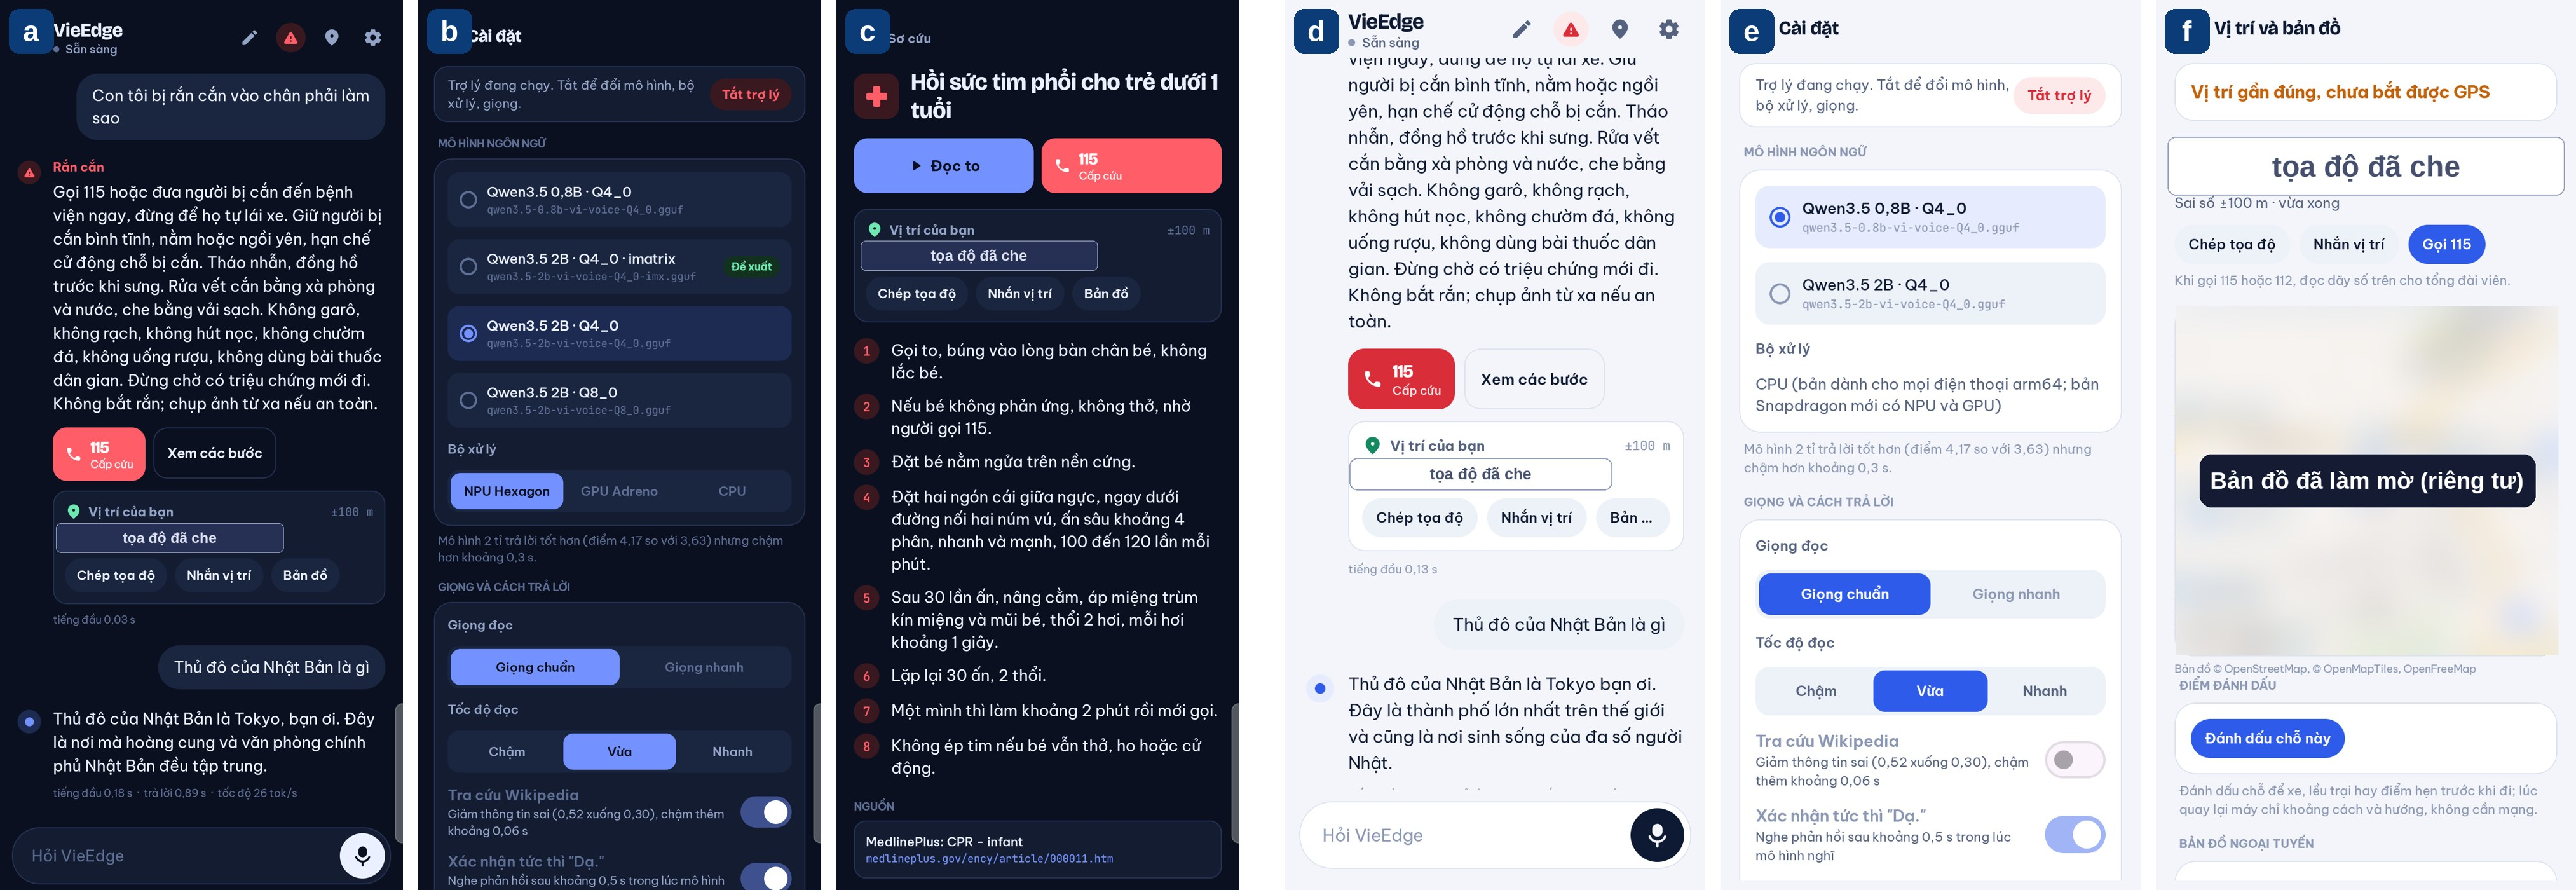
\includegraphics[width=\linewidth]{anh_may.jpg}\par}
{\fontsize{13}{15.5}\selectfont\color{black!75}\textbf{Hình 4.} Ứng dụng chạy trên thiết bị thực: Fold7 (a--c), TCL (d--f).\par}
\end{cotp}\hspace{6mm}%
\begin{minipage}[t][\cao][t]{282mm}\vspace{2.1mm}
\begin{cotp}{282mm}{\caoa}{II. PHƯƠNG PHÁP}
{\centering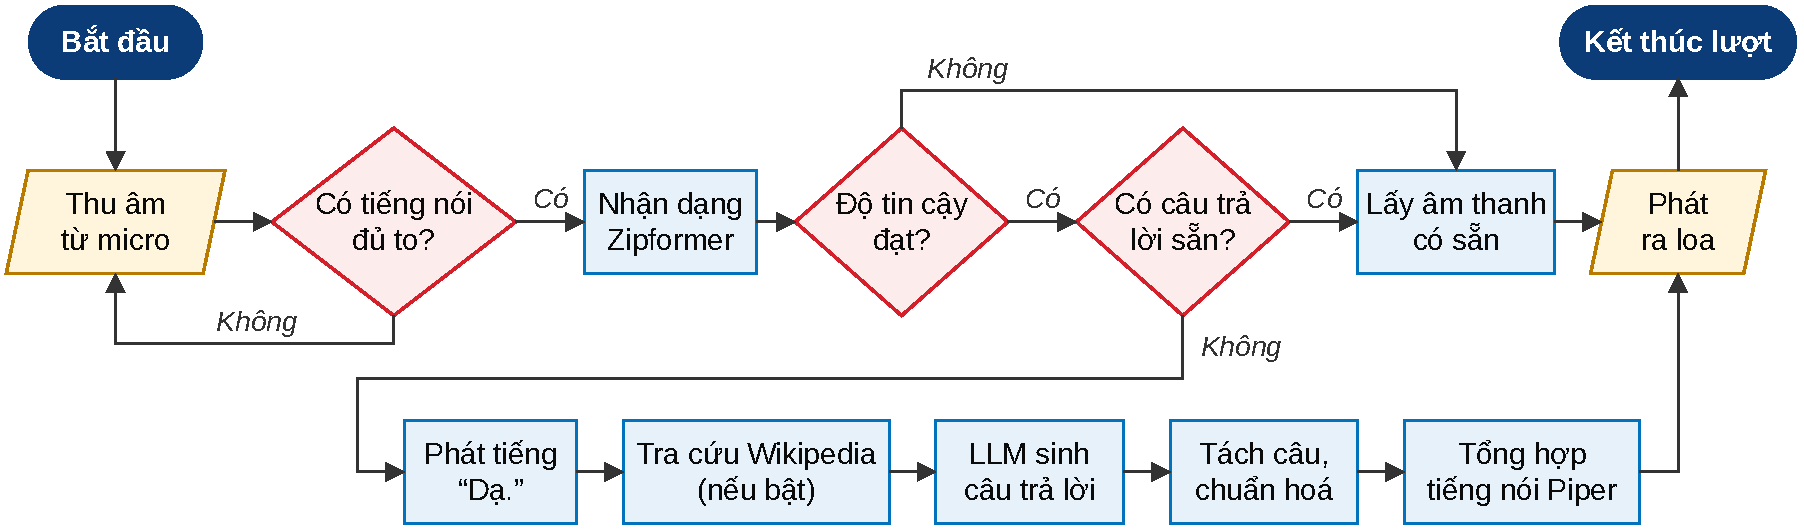
\includegraphics[width=205mm]{luu_do.pdf}\par}
\vspace{4pt}
{\fontsize{17.5}{22}\selectfont
\textbf{\color{dam}Giảm độ trễ:} nhánh nhanh bỏ qua tra cứu, LLM và TTS; cắt câu đầu sau 3 từ; xác nhận ``Dạ.'' chỉ giảm độ trễ cảm nhận. \textbf{\color{dam}Mô hình:} tinh chỉnh LoRA Qwen3.5 0,8 và 2 tỉ tham số; Q4\_0 tận dụng lệnh dotprod, xử lý prompt nhanh hơn 43\%; STT Zipformer [3]; Pi dùng PREEMPT\_RT [4]; tra cứu 200.000 bài Wikipedia.\par}
\end{cotp}

\vspace{4pt}
\begin{cotp}{282mm}{\caob}{III. KẾT QUẢ}
\begin{minipage}[t]{136mm}
\hinh{hai_may_latency.pdf}{122mm}{\textbf{Hình 1.} Pi 5 và hai điện thoại, thang logarit. ``Dạ.'' đưa phản hồi đầu xuống dưới 1\,s trên Fold7; TCL cần 12,6\,s tới nội dung trả lời.}
\end{minipage}\hfill
\begin{minipage}[t]{136mm}
\hinh{stages_v2.pdf}{106mm}{\textbf{Hình 2.} Cơ cấu độ trễ theo chặng, mô hình 0,8 tỉ, tắt tra cứu.}
\hinh{platform_v2.pdf}{100mm}{\textbf{Hình 3.} Tốc độ LLM trên từng nền tảng; NPU xử lý prompt nhanh nên tra cứu gần như không làm tăng độ trễ.}
\end{minipage}
\end{cotp}
\end{minipage}\hspace{6mm}%
\begin{cotk}{\rong}{\cao}
\vspace{4.2mm}\phu{Pi OS và Yocto-RT trên cùng Pi 5}
{\fontsize{16.5}{21}\selectfont\setlength{\tabcolsep}{4pt}\centering
\begin{tabular}{@{}l r r@{}}\toprule
Chỉ số & Pi OS & Yocto-RT\\\midrule
Jitter tải nặng 30 ph (µs) & 127 & \textbf{92}\\
Trả lời, không tải, p50 (s) & 1,60 & 2,02\\
RAM sau khởi động (MB) & 442-538 & \textbf{285}\\
Công suất PMIC, không tải (W) & 3,03 & \textbf{2,78}\\\bottomrule
\end{tabular}\par}
\vspace{3pt}
{\fontsize{16.5}{20}\selectfont So cặp 16 câu: chênh lệch 0,06\,s, $p=0{,}40$. Lợi ích của Yocto-RT là khả năng cô lập, không phải tốc độ suy luận.\par}
\phu{Thẻ an toàn trên tập độc lập}
{\fontsize{16}{20}\selectfont\setlength{\tabcolsep}{4pt}\centering
\begin{tabular}{@{}l r r r@{}}\toprule
Tập (số thẻ) & Văn bản & Giọng rõ & Giọng kém\\\midrule
v3 (60) & 111/114 & 102/114 & 55/114\\
v4 (76) & 64/64 & 47/64 & 28/64\\
v5 (85) & 35/36 & 30/36 & 15/36\\\bottomrule
\end{tabular}\par}
\vspace{2pt}{\fontsize{14.5}{17.5}\selectfont Câu thông thường bị kích hoạt nhầm: 0/20 ở v4, v5. Điểm yếu là nhận dạng giọng nói (WER 0,15 đến 0,44 trên giọng tổng hợp).\par}
\phu{Nhiệt và công suất trên Fold7}
{\fontsize{16.5}{20}\selectfont 7,5 phút, 62 lượt: NPU tối đa 65\,°C, duy trì 25,3 token/s; toàn máy tiêu thụ 2,2 đến 3,3\,W.\par}
\vspace{5pt}
\muc{IV. KẾT LUẬN}
{\fontsize{17.5}{21.5}\selectfont
\begin{itemize}[itemsep=2pt]
\item Đạt phản hồi đầu p95 dưới 1,5\,s (Pi 1,15\,s; Fold7 1,24\,s), 0 xrun, hoàn toàn ngoại tuyến.
\item Câu khẩn cấp được trả lời bằng thẻ có trích dẫn nguồn: 97\% đến 100\% câu văn bản chọn đúng thẻ, LLM không tự sinh lời khuyên y tế.
\item Chạy được trên điện thoại phổ thông 4\,GB RAM (TCL T506T) với cùng độ chính xác; câu khẩn cấp có phản hồi sau \tclSafeMed\,s.
\item Chưa đạt: bộ mã hoá trên Hailo-8L (cosine 0,84). Hạn chế: đo bằng giọng tổng hợp.
\end{itemize}\par}
\vspace{3pt}
{\fontsize{12.5}{15}\selectfont\color{black!75}\textbf{Tài liệu tham khảo.} [1] T. Stivers et al., PNAS 106(26), 2009. [2] T. Likhomanenko et al., ChipChat, arXiv:2509.00078, 2025. [3] Z. Yao et al., Zipformer, ICLR 2024. [4] F. Reghenzani et al., ACM CSUR 52(1), 2019.\par}
\end{cotk}
\end{minipage}
\end{document}
